\FloatBarrier
\begin{figure}[!h]
\centering
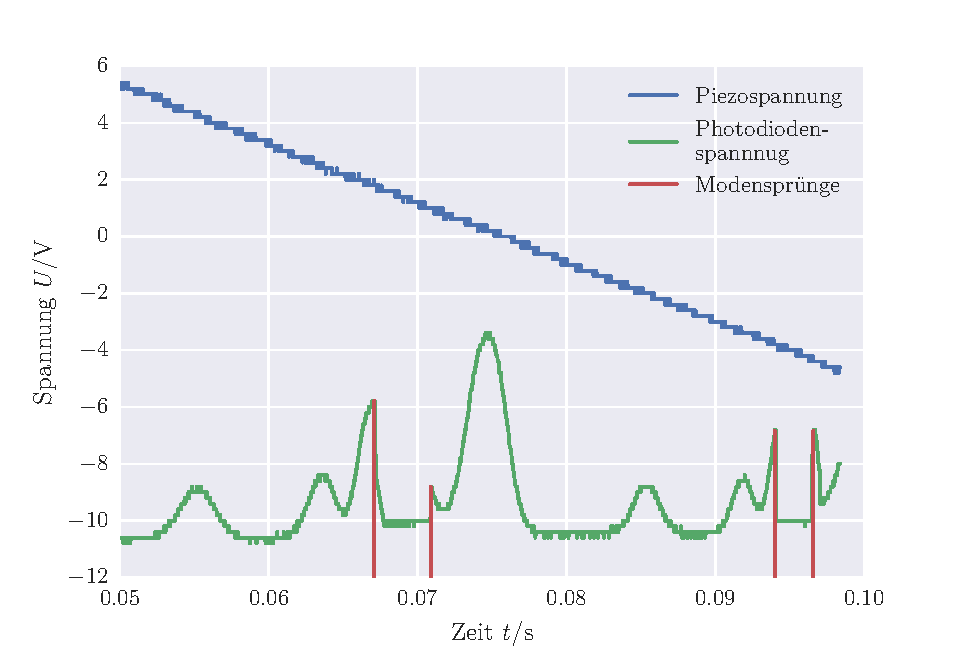
\includegraphics[scale=1]{../Grafiken/Filter_und_NDFilter.pdf}
\caption{Darstellung der vom Oszilloskop aufgenommenen Spannungen.
	 Zu sehen ist zum einen eine abfallende Flanke der an den piezoelektrischen Wandler
	 angeschlossenen Dreiecksspannung. Zum Anderen ist die Spannung der Photodiode abgebildet,
	 an der sich bereits das zu beobachtend Absorptionsspektrum erkennen lässt.
	 Neben den Absorptionsspitzen sind auch die noch vorhandenen Modensprünge deutlich zu 
	 sehen.\label{fig:filter_und_ndfilter}}
\end{figure}
\FloatBarrier